\section{Experiments}
\label{sec:experiments}
We implemented and trained our SAMNet model using MI-Prometheus~\cite{kornuta2018accelerating}, a framework based on Pytorch~\cite{paszke2017automatic}. 
We evaluated the model on the COG dataset~\cite{yang2018dataset}, a video reasoning~\cite{mogadala2019trends} dataset developed for the purpose of research on relational and temporal reasoning, as well as on the CLEVR dataset~\cite{johnson2017clevr}, created for Image Question Answering research.
There are 23 classification question categories in COG and the 5 original question categories in CLEVR.
Our experiments were designed to study SAMNet's performance in terms of generalization and transfer learning abilities in different settings,
and involved incorporating variants of both datasets.  
For COG, the Canonical (easy) and Hard variant differ mainly on the number of frames in the video, 
the maximum amount of look-back in frame history containing relevant information for reasoning, 
and the number of object distractors (see~\cref{tab:cog_variants}).
For CLEVR, we consider the CoGenT (Constrained Generalization Test) variant which contains two conditions, differing on the combinations of attribute values (details in~\cref{sec:temporal}).
%In some of our experiments, we also compare using a \emph{zero-shot learning} approach  for transfer learning to another approach
%involving \emph{finetuning}.
%Recall that the former involves evaluating the trained model of the source directly on the target while for the latter we do additional lightweight 
%training on the target labeled data before evaluating its performance. 
\begin{table}[ht]
	\centering
		\begin{tabular}{lccc}
			\toprule
			Variant	& Frames & History	& Distractors \\ 
			\midrule
			Canonical (Easy) & 4 & 3 & 1\\	
			Hard  & 8 & 7 & 10\\
			\bottomrule	
		\end{tabular}
	\caption{Details of the Canonical and Hard variants of COG.}
	\label{tab:cog_variants}
\end{table}\vspace{5pt}

%More details on the composition of these datasets is available in Appendix \ref{sec:datasets-desc}.

\subsection{Performance of SAMNet vs baseline model~\cite{yang2018dataset}}
\label{sec:cog-baseline-compare}

We trained SAMNet using 8 reasoning steps and external memory of 8 address locations, each storing an array of 128 floats. 
%We have also carried out experiments with different numbers of reasoning steps and memory size, but this goes beyond the scope of this paper.
We compared our results with the baseline model introduced in the same paper as the COG dataset~\cite{yang2018dataset}.
The most important results are highlighted in~\cref{fig:samnet_cog_detailed}; full comparison can be found in the supplementary material.%Appendix~\ref{sec:cog-all-results}.

\begin{figure*}[htb]
	\centering
	\begin{subfigure}{\textwidth}
		\centering
		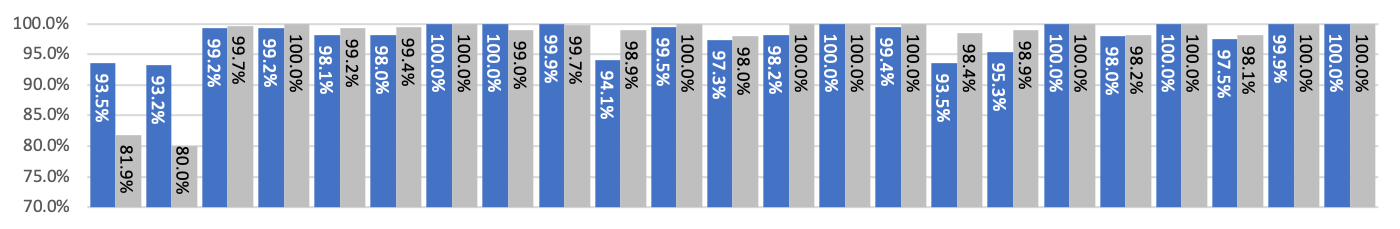
\includegraphics[width=\textwidth]{../img/results/samnet_cog_orig_canonical_no_labels.png}
	\end{subfigure}%
	\newline
	\begin{subfigure}{\textwidth}
		\centering
		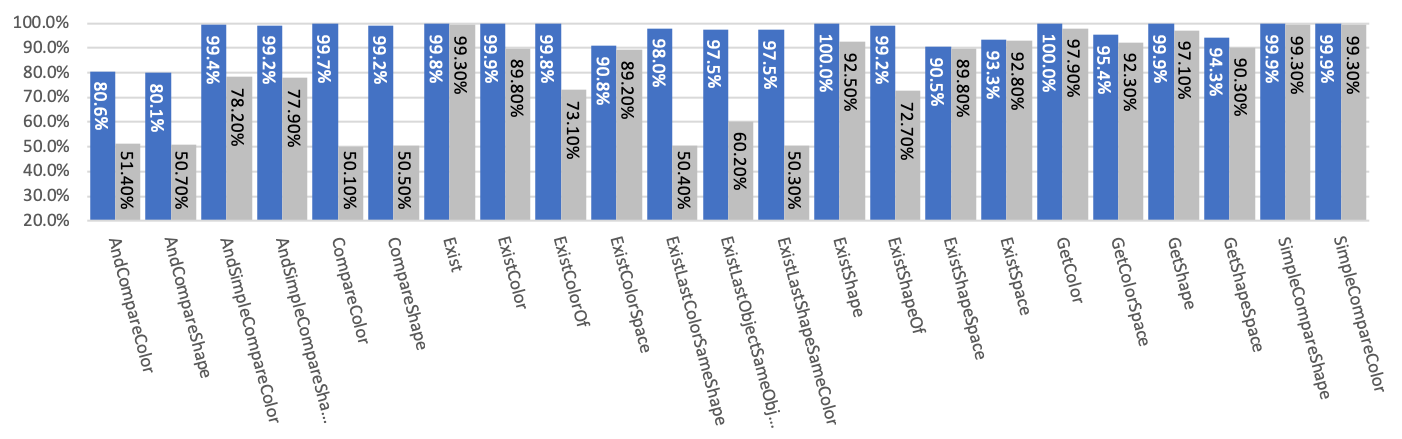
\includegraphics[width=\textwidth]{../img/results/samnet_cog_orig_hard.png}
	\end{subfigure}%
	\caption{Comparison of test set accuracies of SAMNet (blue) with original results achieved by the 
		baseline model~\cite{yang2018dataset} (gray) on Canonical (top) and Hard (bottom) variants of the COG dataset.}
	\label{fig:samnet_cog_detailed}
\end{figure*}

For the Canonical variant (top row), we achieve similar accuracies for the majority of tasks (with a total average accuracy of 98.0\%, 
compared to 97.6\% for the baseline model), with significant improvements (around 13 points) for \textit{AndCompare} tasks.
As these tasks focus on compositional questions referring to two objects, we hypothesize that our model achieves better 
accuracy due to its ability to selectively pick and store relevant objects from the past frames in memory.
For the Hard variant, we achieve a total average accuracy of 96.1\% compared to 80.1\% for the baseline model, demonstrating
that our model can adapt to larger number of frames and distractors.
Despite there being some tasks in the Canonical variant where SAMNet achieved slightly lower accuracies,
% (between 0.2 and 1.8 points)
when comparing performances on the Hard variant, it improves upon the baseline model on all tasks, 
with improvements varying from 0.5 to more than 30 points, and especially on the more complex tasks in the dataset.

\subsection{Reasoning transfer on CLEVR and COG}
\label{sec:reasoning}
In these experiments using the CLEVR and COG datasets, we focus on analyzing the impact 
of each task relative to others using appropriate groupings of tasks.
%For each dataset, we defined appropriate task families that reflect the characteristics of that dataset and designed
%appropriate experiments to study the effectiveness of transfer learning across task families.

\subsubsection{CLEVR}
\label{sec:reasoning-clevr}
For the CLEVR dataset, we consider the question categories defined by the authors: \textit{Exist}, \textit{Count}, \textit{CompareInteger}, \textit{CompareAttribute}, \textit{QueryAttribute}. For performance reasons, we deactivated the external memory and temporally-related modules in SAMNet as they are unnecessary while reasoning about static images. We conduct the following experiments:
\begin{itemize}
	\item Train and test SAMNet on a single task group $t$. These 5 experiments fit into the traditional ML setup of single-task learning;
	\item Train SAMNet on all task groups jointly and evaluate its performance on each task group $t$ separately.
	This is a transfer learning setting where for the source task family, the task is sampled from all questions,
	while for the target task family, the samples consist of questions from group $t$ only;
	\item Finally, for each task group $t$, we train SAMNet on all tasks but $t$, and test its performance on $t$.
	This can also be viewed as a transfer learning setting similar to the previous case.
	%These experiments steer away from single / multi-task training and rather fall under the Domain Adaptation setting, categorized as \emph{transductive} transfer learning in \cite{pan2009survey}.
\end{itemize}

Noticeable results are shown in~\cref{fig:CoGenT-results}, while the complete set is available in the supplementary material.%Appendix \ref{sec:full-cogent-results}.

\begin{figure}[!t]
	\centering
	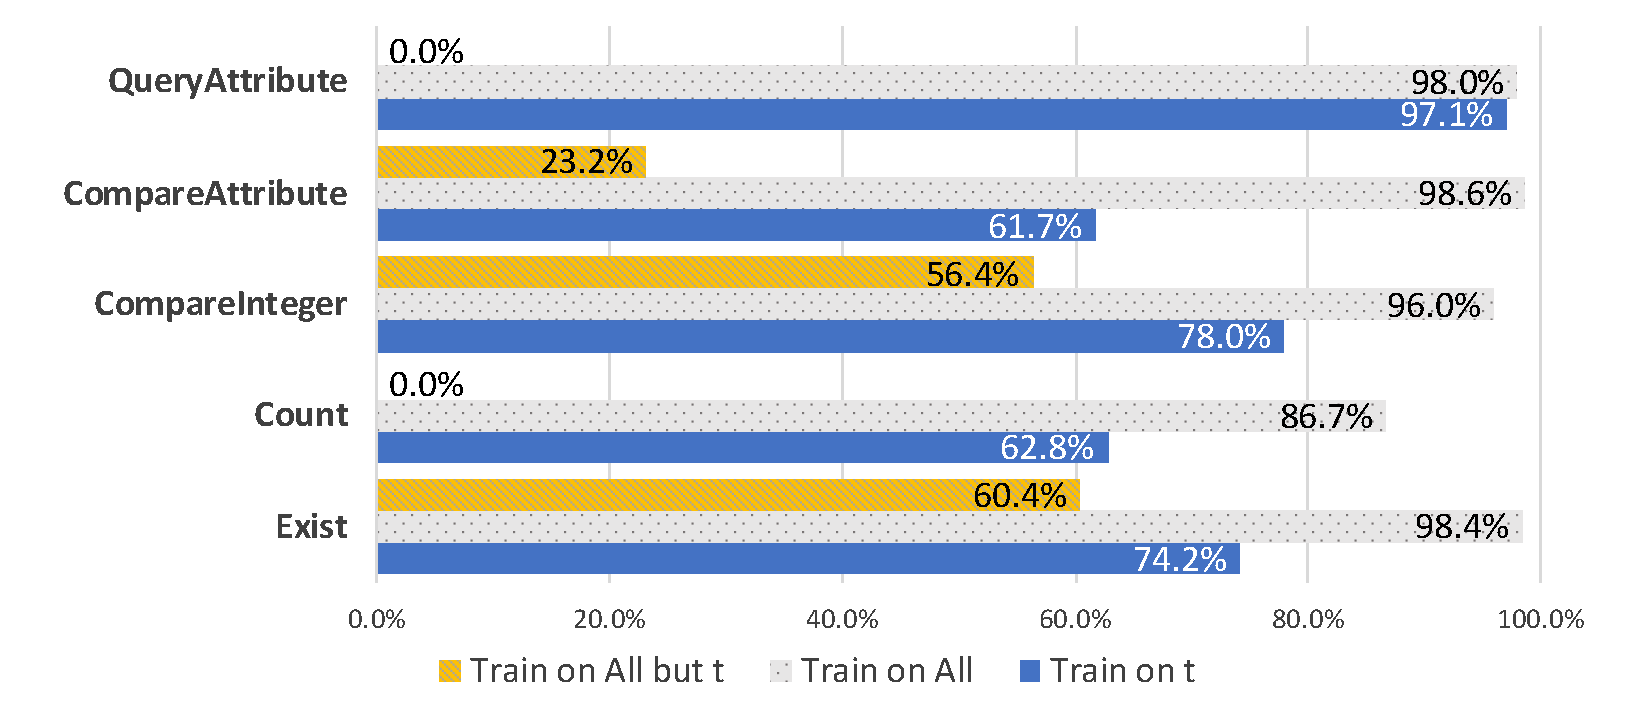
\includegraphics[width=0.8\textwidth]{../img/results/CoGenT_results.pdf}
	\caption{CLEVR-CoGenT accuracies for all tasks $t$ when training on $t$ only, training on all tasks jointly and training on all tasks but $t$.} %For all experiments, the validation and test sets are identical.
	\label{fig:CoGenT-results}
\end{figure}


Looking at~\cref{fig:CoGenT-results}, SAMNet does well on \textit{Count} and \textit{QueryAttribute}, but poorer on the 3 other tasks in the single-task learning setting (blue). Indeed, \textit{Exist}, \textit{CompareInteger} and \textit{CompareAttribute} are binary tasks; \textit{Count} has output labels digits 0 through 10 (so $<$10\% accuracy by chance) and \textit{QueryAttribute} maps to the set of object-attribute values (15 labels).

Nevertheless, significant accuracy gains are noted when training jointly on all tasks (gray), ranging from 18 points to 37 points on 4 out of 5 tasks. These improvements suggest that related tasks benefit from joint training. \textit{QueryAttribute} only sees an increase of one point. One could qualify it as \textit{self-sufficient} as it does not appear to benefit from joint training with other tasks. 
%We plan to run additional experiments to jointly train on $t$ and all possible subsets of the remaining 4 tasks ($2^4$ experiments per task). We hypothesize that the improvements on e.g. \textit{Exist} would mostly originate from training jointly on \textit{CompareAttribute} and \textit{CompareInteger} since all 3 tasks share the same output space (i.e., labels domain).

Finally, the ``all-tasks-but-$t$'' experiments (yellow) demonstrate that while tasks are related, one does not subsume another in terms of learning. Indeed, we can observe that for \textit{CompareAttribute}, while \textit{Exist} and \textit{CompareInteger} share the same output space, including them and holding out \textit{CompareAttribute} from the training set results in poor accuracy.
We also observe no learning for \textit{Count} and \textit{QueryAttribute}. As these categories have labels that do not overlap with other categories, the model cannot predict these labels.


An additional set of experiments, for which results are available in the supplementary material,
%Appendix \ref{sec:full-cogent-results}
fine-tune the model trained on all tasks on each task $t$ respectively.
%Given the initial training on all tasks, we were interested in the tradeoff between the performance gain, if any, on the fine-tuned task and the drop, if any, on other tasks.
Fine-tuning did not demonstrate a clear benefit (except for \textit{Count}, where the accuracy increased by 1.5 pt) without hurting performance on the other tasks. Nevertheless, these experiments leave open the possibility that joint training of tasks may potentially benefit from using weighted sampling towards the tail end with more emphasis on samples from less performing task groups, similar to~\cite{guo2018dynamic, kendall2018multi}.

\subsubsection{COG}
\label{sec:reasoning-cog}
Since the number of task classes (=23) in the COG dataset is large, we designed a 2-level hierarchy of task groups using the
description of these tasks, as shown in~\cref{fig:task-groups}.

\begin{figure}[!t]
	\centering
	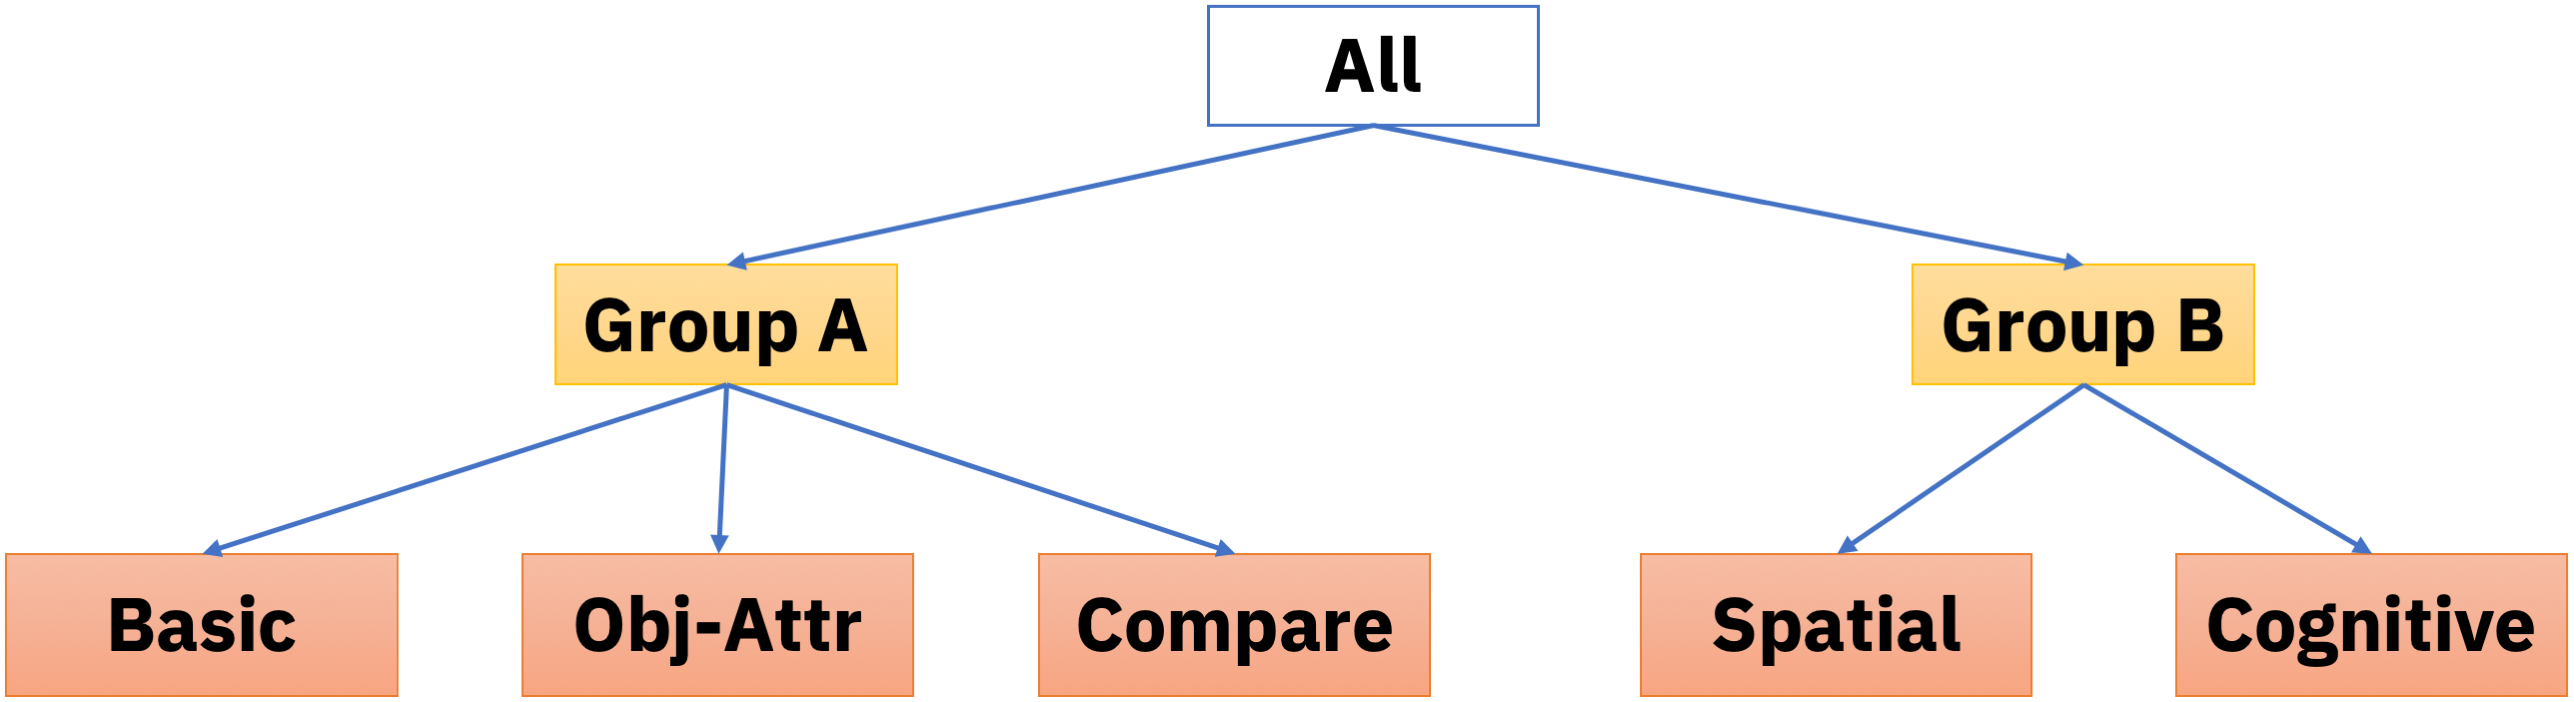
\includegraphics[width=0.8\textwidth]{../img/architecture/hierarchy}
	\caption{Hierarchy of Task Groups.}
	\label{fig:task-groups}
\end{figure}

\bigskip

For groups at the lowest level, we chose the following task classes to be placed in those groups.
Below, substitute each of \textit{Shape} and \textit{Color} for  \uX{} to obtain the task class.
\begin{description}
	\item[Basic:] \textit{Exist}\uX, \textit{Get}\uX{} and \textit{Exist};
	\item[Obj-Attr:] \emph{SimpleCompare}\uX{} and \textit{AndSimpleCompare}\uX;
	\item[Compare:] \textit{Compare}\uX,  \textit{AndCompare}\uX{} \& \textit{Exist}\uX\textit{Of};
	\item[Spatial:] \textit{ExistSpace}, \textit{Exist}\uX\textit{Space}, and \textit{Get}\uX\textit{Space};
	\item[Cognitive:] \textit{ExistLastColorSameShape}, \textit{ExistLastShapeSameColor} and \textit{ExistLastObjectSameObject}
\end{description}

\begin{figure}[!t]
	\centering
	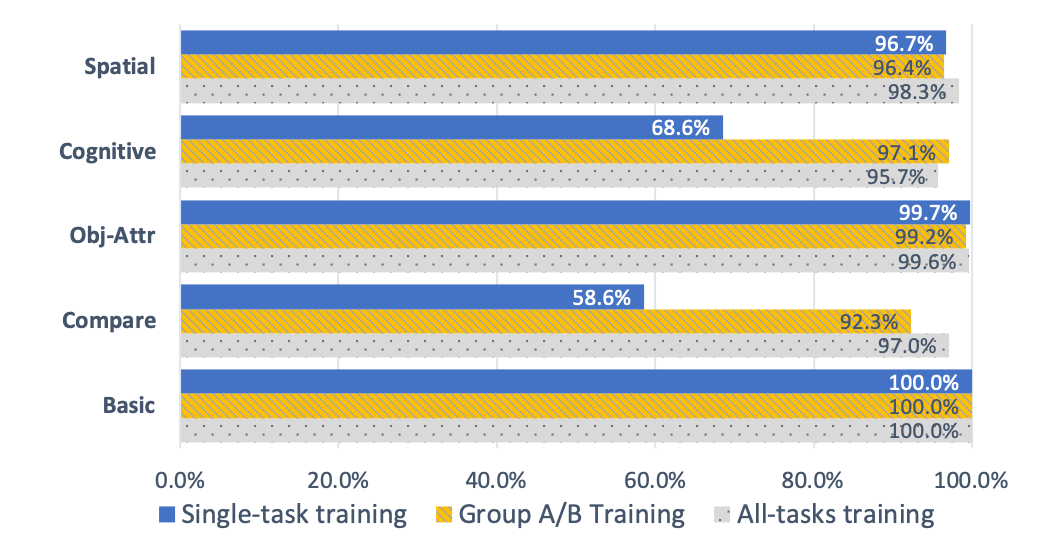
\includegraphics[width=0.85\textwidth]{../img/results/COG_reasoning_transfer_v3}
	\caption{COG accuracies for all task groups $t$ when training on $t$ only; training on Group A or B; and on all tasks.}
	\label{fig:COG-reasoning-results}
\end{figure}

We then conducted the following experiments using the Canonical variant of COG to study 
whether transfer learning was effective in leveraging information gained by training a task family at a higher level
of the hierarchy:
 \begin{itemize}
	\item Train and test SAMNet on each of the 5 task groups at the lowest level of the hierarchy (Single-task training);
	\item Jointly train on:
	\begin{itemize}
		\item 	 \textbf{Group A} and test on each task from the lowest groups (i.e. \textbf{Basic}, \textbf{Obj-Attr} and \textbf{Compare}) separately;
		\item \textbf{Group B} and test separately on \textbf{Spatial} and \textbf{Cognitive};
	\end{itemize}
	\item As a baseline, we compared the above results to the earlier experiment shown in~\cref{fig:samnet_cog_detailed}, which
	can be viewed as training jointly on \textbf{All} and testing on each group at the leaf level separately (All-task training).
\end{itemize}

The results of these experiments are shown in~\cref{fig:COG-reasoning-results}.

First, notice that for each of the \textbf{Basic} and \textbf{Obj-Attr} task families, the accuracy is near-perfect in all cases, suggesting that each contains the most primitive tasks and therefore do not benefit from training with other task families.
With \textbf{Spatial}, we see a small improvement showing that there is some benefit due to joint training with other task families.
Two groups that demonstrated a huge improvement of more than 25 points are \textbf{Compare} and \textbf{Cognitive}.
The former saw an accuracy jump from 68.6\% by training on samples from that family alone
to 97.0\% when training on all samples. To further emphasize this behavior, notice that 
just joining \textbf{Compare} with \textbf{Obj-Attr} and \textbf{Basic} already causes a significant accuracy jump to 92.3\%. 
In hindsight, this is not surprising, as the questions in \textbf{Compare} are composed
of fragments of questions given by \textbf{Basic} and \textbf{Obj-Attr}, and therefore can leverage the reasoning strategies developed there to reason about questions in \textbf{Compare}.
Lastly, for the \textbf{Spatial} family, we again see the benefits of joint training with all questions (68.6\% to 95.7\%) but in this case there
is a slight loss incurred by including everything. As seen in the figure, just jointly training with \textbf{Spatial} alone is sufficient to get a boost in accuracy (97.1\%). To summarize, while joint training helps, one needs to determine how much of correlation is present with the other tasks.

  

\subsection{Temporal transfer in COG}
\label{sec:temporal}

The goal here is to test the transfer learning ability concerning the frame sequence length, frame history required
for reasoning, and the number of object distractors.
For that purpose, we compare both models when trained on the Canonical variant but tested on the 
Hard variant (\cref{fig:samnet_cog_overall_transfer}).
The light gray color indicates original accuracies of the baseline model from paper, 
whereas dark gray indicates accuracies of the baseline model
obtained by running the original code provided by the authors~\cite{yang2018implement}.

The first column displays the scores of the traditional ML setup when training and testing on the Canonical variant. 
The observed close scores in light and dark gray underscore the baseline model reproducibility.
For both cases of zero-shot learning (second column--91.6\% vs 65.9\%) and fine-tuning using a single epoch 
(third column--96.7\% vs. 78.1\%), SAMNET outperforms the baseline model significantly.
Interestingly, this fine-tuning yields a mild boost of +0.6\% on the earlier reported accuracy 
in~\cref{sec:cog-baseline-compare} (fourth column).
These results suggest that it suffices to train SAMNet on simpler videos 
to enable learning of good memory usage and attention on relevant entities  
in order to achieve comparable, if not better, 
performance on longer video frames with more complex scenes.

\begin{figure}[htb]
	\centering
	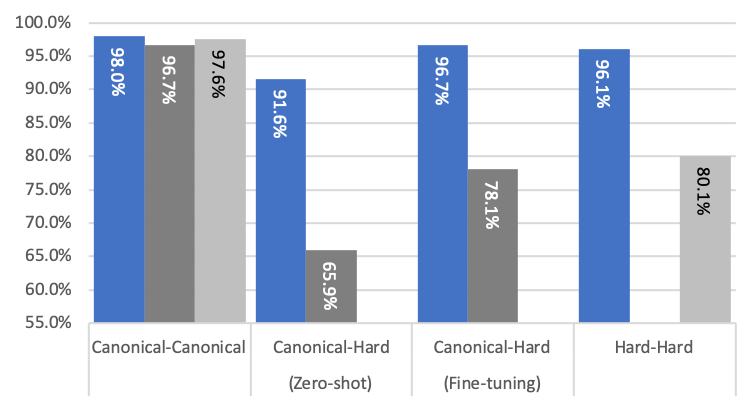
\includegraphics[width=0.8\textwidth]{../img/results/samnet_cog_overall_transfer.png}
	\caption{Total accuracies of SAMNet (blue) and baseline models (light/dark gray) when testing generalization from Canonical to Hard variants of the dataset.}
	\label{fig:samnet_cog_overall_transfer}
\end{figure}


\subsection{Feature transfer on CLEVR-CoGenT}
\label{sec:feature}
\begin{table}[ht]
	\centering
	%\begin{adjustbox}{width=0.45\textwidth}
		\begin{tabular}{cccc}
			\toprule
			Dataset	& Cubes	& Cylinders &	Spheres	\\
			\midrule
			CoGenT A &  Family A  & Family B 	&	Any color  \\
			CoGenT B	&	Family B  &	Family A	&	Any color \\
			\bottomrule
		\end{tabular}
	%\end{adjustbox}
	\caption{Restrictions on feature combinations in A \& B conditions of the CoGenT variant of the CLEVR dataset.}
	\label{tab:cogent_conditions}
\end{table}

The final set of experiments we consider is related to feature transfer.
The CoGenT-A \& -B variants of CLEVR differ by the available combinations of 8 object color-attributes.
The colors are partitioned into two complementary families: 
Gray, Blue, Brown and Yellow in \textbf{Family A} and Red, Green, Purple, Cyan in \textbf{Family B}. 
The cubes and cylinders take colors from complementary families in each variant with opposite configurations while the spheres can take any color (See~\cref{tab:cogent_conditions}). 
As the input domain consist of the set of objects with all attribute values, both variants differ by their marginal distributions $P_S$ and $P_T$.
We conduct 2 experiments with SAMNet trained on CoGenT-A:
\begin{itemize}
\item an immediate test (zero-shot learning) from A to B; and 
\item fine-tuning for a single epoch on 30k samples from CoGenT-B (following~\cite{johnson2017inferring, mascharka2018transparency, perez2018film, marois2018transfer}).
\end{itemize}

\begin{figure}[!t]
	\centering
	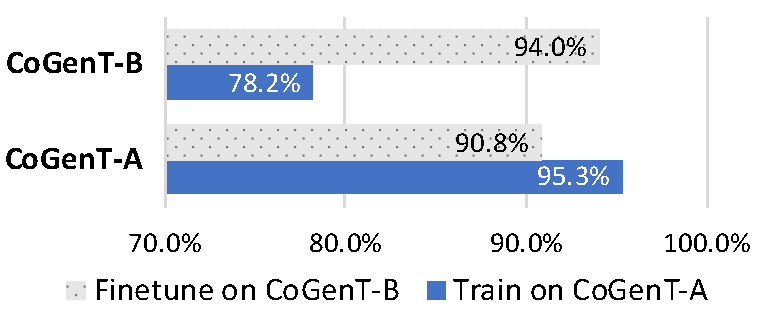
\includegraphics[width=0.6\textwidth]{../img/results/CoGenT_B_results.pdf}
	\caption{Test accuracy on CoGenT-A \& -B when training on CoGenT-A (blue) and fine-tuning on CoGenT-B (gray).}
	\label{fig:CoGenT-B-results}
\end{figure}

Performance of SAMNet on CoGenT (\cref{fig:CoGenT-B-results}) is clearly worse on CoGenT-B than CoGenT-A.
Fine-tuning for a single epoch allows an observable increase of 15 pts on CoGenT-B, and a slight drop on CoGenT-A.
Both are consistent with findings from the literature~\cite{johnson2017inferring, mascharka2018transparency, perez2018film}.
